\chapter{Protocollo di aggregazione simil prio3 utilizzando tecniche omomorfiche}

\section{Introduzione}
Prio3 VDAF \`e, in modo molto semplice, un protocollo pensato per raccogliere dati da pi\`u client e calcolarne un risultato aggregato senza esporre il contributo individuale di ciascuno \cite{prio}. L'idea generale \`e che ogni client non invii direttamente il proprio valore in chiaro a un unico soggetto, ma produca una rappresentazione adatta a essere elaborata da pi\`u attori del protocollo. In questo modo, il sistema finale pu\`o recuperare il risultato complessivo senza ricostruire facilmente il dato del singolo partecipante.

L'obiettivo di questo capitolo \`e allora il seguente: replicare in ambiente FHE la forma generale di un protocollo di aggregazione ispirato a Prio3, mantenendo l'idea di fondo di raccolta privata e di validazione dei report, ma semplificando l'architettura. La costruzione che introduciamo, chiamata \texttt{fhe-vdaf}, usa lo schema omomorfico BGV: i report vengono cifrati dai client, inviati a un unico aggregatore, validati sotto cifratura e poi sommati, in modo che l'attore finale possa apprendere soltanto il risultato aggregato.

La scelta di BGV non \`e casuale. In questo contesto i report sono valori interi e tutta la logica di validazione viene espressa tramite aritmetica modulare. BGV \`e quindi naturale perch\'e lavora direttamente su interi modulo $p$. Questo significa che somme e moltiplicazioni avvengono nello stesso ambiente algebrico in cui vogliamo controllare i report, compreso il comportamento di overflow, che viene assorbito in modo coerente dalla riduzione modulo $p$.

\section{Idea generale di \texttt{fhe-vdaf}}
La struttura di \texttt{fhe-vdaf} pu\`o essere descritta in modo molto semplice:
\begin{enumerate}
  \item il client vuole inviare un valore numerico;
  \item lo converte in una rappresentazione binaria a slot;
  \item cifra tale rappresentazione con la chiave pubblica del sistema;
  \item invia il ciphertext all'aggregatore;
  \item l'aggregatore valida omomorficamente il report;
  \item se il report \`e valido, lo aggiunge alla somma aggregata;
  \item il collector finale decifra solo il totale.
\end{enumerate}

In pratica, tutti i report cifrati arrivano allo stesso aggregatore. La crittografia di base resta la stessa, ma cambia il modo in cui il sistema distribuisce i compiti e la fiducia tra gli attori.

\section{Ruoli architetturali e gestione delle chiavi}

\begin{figure}[H]
\centering
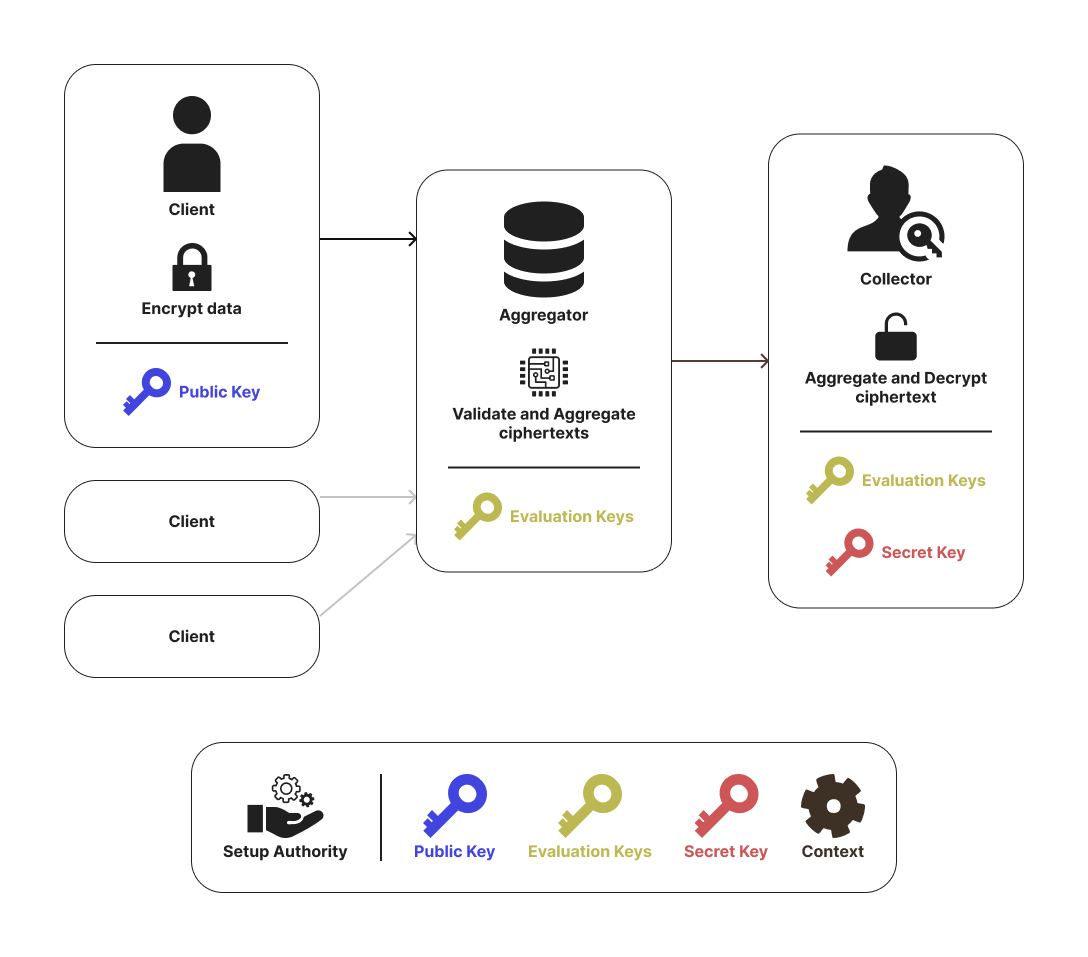
\includegraphics[width=0.95\textwidth]{figures/vdaf_0.png}
\caption{Schema di fhe-vdaf.}
\label{fig:vdaf_0}
\end{figure}

\subsection{Attori del sistema}
Nel caso di \texttt{fhe-vdaf} si possono distinguere quattro attori principali:
\begin{itemize}
  \item il \emph{setup authority}, che crea il contesto crittografico e le chiavi;
  \item i \emph{client};
  \item l'\emph{aggregator}, che riceve i report cifrati;
  \item il \emph{collector}, che decifra il risultato finale.
\end{itemize}

\subsection{Chi possiede quali chiavi}
Dal punto di vista della gestione delle chiavi, \texttt{fhe-vdaf} conserva la distinzione tra cifratura, valutazione omomorfica e decifratura finale.

La distribuzione tipica \`e la seguente:
\begin{itemize}
  \item i \textbf{client} possiedono il contesto pubblico e la \textbf{chiave pubblica} $pk$, necessaria per cifrare i report;
  \item l'\textbf{aggregator} possiede il contesto crittografico e le \textbf{evaluation keys}, cio\`e le chiavi ausiliarie per eseguire somme, rotazioni e moltiplicazioni omomorfiche;
  \item il \textbf{collector} possiede la \textbf{chiave segreta} $sk$ e pu\`o decifrare il risultato finale;
  \item il \textbf{setup authority} genera inizialmente $pk$, $sk$ ed evaluation keys, e poi le distribuisce ai ruoli autorizzati.
\end{itemize}

Questa separazione \`e importante. L'aggregatore pu\`o elaborare i dati cifrati ma, in condizioni normali, non pu\`o decifrarli. Il collector pu\`o decifrare, ma non riceve i singoli report in chiaro durante la fase di raccolta.

\subsection{Conseguenze di sicurezza}
L'aspetto pi\`u delicato di \texttt{fhe-vdaf} \`e la concentrazione dello schema presso l'aggregatore. Questo comporta che:
\begin{itemize}
  \item tutti i ciphertext passano per lo stesso nodo;
  \item tutta la validazione viene eseguita nello stesso punto;
  \item non c'\`e ridondanza fiduciaria tra aggregatori distinti;
  \item un'eventuale collusione tra aggregatore e soggetto che controlla la chiave segreta comprometterebbe la protezione dei report individuali.
\end{itemize}

Per questo motivo, \texttt{fhe-vdaf} \`e molto semplice da capire, ma meno forte di una soluzione con pi\`u aggregatori indipendenti.

\section{Architettura complessiva in uno scenario di dati aggregati}
In \texttt{fhe-vdaf}, tutti i report vengono cifrati e inviati all'aggregatore. L'aggregatore non deve conoscere il contenuto di ciascun numero, ma deve poter:
\begin{itemize}
  \item verificare che ogni report sia ben formato;
  \item scartare i report invalidi;
  \item sommare i report validi.
\end{itemize}

Infine, il collector riceve la somma cifrata finale e la decifra, ottenendo solo il totale aggregato.

\subsection{Schema dei messaggi}
Lo schema architetturale pu\`o essere rappresentato cos\`i, assumendo che il setup authority distribuisca preventivamente le chiavi ai vari attori autorizzati:
\begin{align}
&\text{Client}_i \longrightarrow \text{Aggregator}: \mathsf{Enc}_{pk}(\text{report}_i), \\
&\text{Aggregator}: \text{validate-or-zero}(\mathsf{Enc}_{pk}(\text{report}_i)), \\
&\text{Aggregator}: \sum_i \mathsf{Enc}_{pk}(\text{report}_i), \\
&\text{Aggregator} \longrightarrow \text{Collector}: \mathsf{Enc}_{pk}(\text{totale}), \\
&\text{Collector}: \mathsf{Dec}_{sk}(\mathsf{Enc}_{pk}(\text{totale})).
\end{align}


\section{Conversione dell'input in binario}
\subsection{Perch\'e usare una rappresentazione binaria}
Il cuore operativo del protocollo \`e la trasformazione del dato numerico in una sequenza di slot binari. Questa scelta non \`e un dettaglio marginale: \`e proprio ci\`o che consente all'aggregatore di verificare, anche sotto cifratura, che il report abbia una forma lecita.

La scomposizione in bit permette di ridurre il controllo a una propriet\`a locale:
\begin{equation}
x \in \{0,1\}.
\end{equation}

\subsection{Vincolo sul valore massimo}
Nel prototipo considerato, il valore massimo consentito \`e
\begin{equation}
\texttt{MAX\_SIZE} = 100.
\end{equation}

Per rappresentare correttamente tutti i valori interi compresi tra $0$ e \texttt{MAX\_SIZE}, il numero minimo di bit richiesto si calcola con
\begin{equation}
\texttt{MAX\_BITS} = \lfloor \log_2(\texttt{MAX\_SIZE}) \rfloor + 1,
\end{equation}
valida per $\texttt{MAX\_SIZE} > 0$.

Nel nostro caso:
\begin{equation}
\lfloor \log_2(100) \rfloor + 1 = \lfloor 6.64\ldots \rfloor + 1 = 6 + 1 = 7.
\end{equation}
Quindi
\begin{equation}
\texttt{MAX\_BITS} = 7.
\end{equation}

La codifica non \`e una rappresentazione binaria standard perfettamente uniforme. I primi sei slot usano i pesi classici
\begin{equation}
1,\ 2,\ 4,\ 8,\ 16,\ 32,
\end{equation}
mentre l'ultimo slot usa il peso
\begin{equation}
37.
\end{equation}

La ragione \`e che si vuole far corrispondere il vettore di tutti uno al valore massimo $100$:
\begin{equation}
1 + 2 + 4 + 8 + 16 + 32 + 37 = 100.
\end{equation}

In questo modo, tutti i valori ammessi tra $0$ e $100$ possono essere rappresentati con sette slot binari.

La logica di codifica seguita dal codice \`e la seguente. Si considerano prima i primi sei bit, che possono rappresentare direttamente tutti i valori compresi tra $0$ e
\begin{equation}
\texttt{LOW\_BITS\_MAX\_VALUE} = 2^{6}-1 = 63.
\end{equation}

Se il valore da codificare soddisfa
\begin{equation}
v \leq 63,
\end{equation}
allora viene codificato normalmente nei primi sei bit e l'ultimo bit resta a zero.

Se invece
\begin{equation}
v > 63,
\end{equation}
allora il codice:
\begin{enumerate}
  \item pone l'ultimo bit uguale a $1$;
  \item sottrae il suo peso, cio\`e $37$, dal valore originale;
  \item codifica il valore rimanente nei primi sei bit.
\end{enumerate}

Il valore finale decodificato sar\`a quindi sempre
\begin{equation}
v = v_{\text{low}} + 37 \cdot b_7.
\end{equation}

\subsection{Esempi di codifica}
Un esempio pi\`u interessante \`e un valore maggiore di $63$, ad esempio $64$. In questo caso il codice accende l'ultimo bit e poi codifica il resto:
\begin{equation}
64 - 37 = 27.
\end{equation}
Poich\'e
\begin{equation}
27 = 1 + 2 + 8 + 16,
\end{equation}
si ottiene
\begin{equation}
64 \longmapsto [1,1,0,1,1,0,1].
\end{equation}

Infine, il valore massimo:
\begin{equation}
100 \longmapsto [1,1,1,1,1,1,1].
\end{equation}
Infatti, in questo caso:
\begin{equation}
100 - 37 = 63,
\end{equation}
e $63$ viene rappresentato dai primi sei bit tutti a uno:
\begin{equation}
63 = 1 + 2 + 4 + 8 + 16 + 32.
\end{equation}

\section{Validazione omomorfica dell'input}
\subsection{Controllo che ogni slot sia un bit}
Una volta ricevuto un ciphertext, l'aggregatore deve verificare che ogni slot codifichi davvero un bit, cio\`e un valore $0$ oppure $1$.

Il controllo fondamentale usa il polinomio elementare
\begin{equation}
f(x) = x(x-1).
\end{equation}

Quindi:
\begin{itemize}
  \item se uno slot contiene $0$ o $1$, il controllo restituisce zero;
  \item se contiene un altro valore, compare un errore non nullo.
\end{itemize}

Se il ciphertext contiene gli slot $x_1,\dots,x_{\texttt{MAX\_BITS}}$, l'aggregatore calcola per ogni slot
\begin{equation}
e_i = x_i(x_i-1)
\end{equation}
e poi somma tutti gli errori:
\begin{equation}
E = \sum_{i=1}^{\texttt{MAX\_BITS}} e_i.
\end{equation}

Se il report \`e ben formato, allora
\begin{equation}
E = 0.
\end{equation}
Se invece almeno uno slot non \`e binario, allora
\begin{equation}
E \neq 0.
\end{equation}

\subsection{Da errore a flag di validit\`a}
Il valore $E$ \`e ancora cifrato. L'aggregatore non pu\`o leggerlo direttamente, ma pu\`o trasformarlo in un flag di errore sfruttando l'aritmetica del campo finito usato dallo schema BGV.

Nel prototipo viene usato il modulo primo
\begin{equation}
p = 786433.
\end{equation}

Per il piccolo teorema di Fermat, per ogni elemento non nullo vale
\begin{equation}
E^{p-1} = 1 \pmod p,
\end{equation}
mentre se $E=0$ allora
\begin{equation}
E^{p-1} = 0.
\end{equation}

Poich\'e
\begin{equation}
p-1 = 786432 = 3 \cdot 2^{18},
\end{equation}
l'aggregatore pu\`o costruire il flag di errore come
\begin{equation}
\text{is\_error} = E^{786432}.
\end{equation}

Il significato \`e:
\begin{itemize}
  \item $\text{is\_error}=0$ se il report \`e valido;
  \item $\text{is\_error}=1$ se il report \`e invalido.
\end{itemize}

Da qui si ottiene il flag opposto:
\begin{equation}
\text{is\_ok} = 1 - \text{is\_error}.
\end{equation}

Quindi:
\begin{itemize}
  \item $\text{is\_ok}=1$ per i report validi;
  \item $\text{is\_ok}=0$ per i report invalidi.
\end{itemize}

\subsection{Validate-or-zero}
A questo punto l'aggregatore moltiplica il report cifrato per il flag di validit\`a:
\begin{equation}
\text{report}_{\text{checked}} = \text{report} \cdot \text{is\_ok}.
\end{equation}

Il risultato \`e molto intuitivo:
\begin{itemize}
  \item se il report \`e valido, viene moltiplicato per $1$ e resta invariato;
  \item se il report \`e invalido, viene moltiplicato per $0$ e diventa il vettore nullo.
\end{itemize}

Questa tecnica \`e spesso descritta come \emph{validate-or-zero}. In un prototipo dimostrativo \`e utile perch\'e consente di continuare l'aggregazione senza interrompere l'esecuzione per ogni input scorretto.

\section{Aggregazione dei report validi}
Una volta validati tutti i report, l'aggregatore li somma omomorficamente. Se i report validi sono $c_1,\dots,c_m$, la somma aggregata \`e
\begin{equation}
C_{\text{sum}} = c_1 + c_2 + \cdots + c_m.
\end{equation}

Poich\'e ogni ciphertext contiene i sette slot della codifica binaria, il risultato della somma \`e un nuovo vettore cifrato i cui slot rappresentano la somma posizione per posizione dei bit validi ricevuti.

Il collector riceve questo ciphertext finale e lo decifra. Dopo la decifratura, non ottiene direttamente il totale come singolo intero, ma i sette slot aggregati:
\begin{equation}
[s_1,s_2,s_3,s_4,s_5,s_6,s_7].
\end{equation}

Il totale finale viene quindi ricostruito come
\begin{equation}
\text{totale} =
1\cdot s_1 +
2\cdot s_2 +
4\cdot s_3 +
8\cdot s_4 +
16\cdot s_5 +
32\cdot s_6 +
37\cdot s_7.
\end{equation}

Questo passaggio \`e analogo alla funzione di \emph{decode} del valore usata nel progetto.

\section{Esempio completo su dati aggregati}
\subsection{Codifica dei valori}
La codifica binaria a sette slot produce:
\begin{align}
51 &\longmapsto [1,1,0,0,1,1,0], \\
7 &\longmapsto [1,1,1,0,0,0,0], \\
4 &\longmapsto [0,0,1,0,0,0,0], \\
49 &\longmapsto [1,0,0,0,1,1,0], \\
13 &\longmapsto [1,0,1,1,0,0,0].
\end{align}

Ogni vettore viene cifrato con la chiave pubblica $pk$ e inviato all'aggregatore.

\subsection{Somma per slot}
Dopo la decifratura, il collector ottiene la somma per slot:
\begin{equation}
[4,2,3,1,2,2,0].
\end{equation}

\subsection{Decodifica finale}
Il totale finale si ricostruisce come:
\begin{align}
\text{totale}
&= 1\cdot 4 + 2\cdot 2 + 4\cdot 3 + 8\cdot 1 + 16\cdot 2 + 32\cdot 2 + 37\cdot 0 \\
&= 4 + 4 + 12 + 8 + 32 + 64 + 0 \\
&= 124.
\end{align}

Il collector apprende dunque solo il totale
\begin{equation}
124,
\end{equation}
senza aver partecipato alla validazione dei singoli report e senza aver ricevuto i report individuali in chiaro durante la fase di raccolta.

\section{Punti di forza e limiti architetturali}
L'architettura adottata presenta una serie di vantaggi pratici, ma anche limiti precisi che vanno esplicitati con chiarezza.

\subsection{Vantaggi}
I vantaggi principali di \texttt{fhe-vdaf} sono:
\begin{itemize}
  \item semplicit\`a architetturale;
  \item minore complessit\`a di orchestrazione;
  \item minore frammentazione degli artifact e dei flussi;
  \item facilit\`a di integrazione in sistemi centralizzati.
\end{itemize}

\subsection{Limiti}
I principali limiti sono:
\begin{itemize}
  \item assenza di distribuzione fiduciaria tra aggregatori distinti;
  \item concentrazione di tutti i ciphertext presso lo stesso nodo;
  \item maggiore esposizione in caso di compromissione dell'aggregatore;
  \item minore vicinanza alle costruzioni VDAF pi\`u robuste.
\end{itemize}

\section{Conclusioni}
\texttt{fhe-vdaf} pu\`o essere visto come una forma molto semplice di raccolta privata di conteggi basata su cifratura omomorfica e validazione VDAF-like. Il meccanismo centrale \`e quello della codifica binaria del valore, del controllo elementare di validit\`a e dell'aggregazione cifrata presso un unico nodo.

Il capitolo ha evidenziato tre aspetti principali. Il primo riguarda l'architettura: client, aggregatore unico e collector con chiavi chiaramente separate. Il secondo riguarda la codifica dell'input, che trasforma ogni valore ammesso in un vettore di bit pesati. Il terzo riguarda la validazione, basata su controlli polinomiali elementari ma molto efficaci per riconoscere valori non binari.

In uno scenario reale, questa architettura pu\`o essere utile come base sperimentale o come soluzione centralizzata per aggregazioni relativamente semplici. Resta per\`o importante ricordare che la semplicit\`a di \texttt{fhe-vdaf} corrisponde anche a una minore distribuzione del trust. Di conseguenza, il suo impiego va valutato nel quadro pi\`u ampio della governance del sistema, della gestione delle chiavi e delle garanzie organizzative offerte dall'infrastruttura che lo ospita.
